\chapter{Implementación}

A continuación se detallan la instalación, configuración así como el desarrollo de los elementos que componenen el sistema. A modo de resumen los puntos serán los siguientes:

\begin{itemize}
	\item Descripción de las tecnologías seleccionadas.
	\item Instalación y configuración de Raspberry Pi.
	\item Instalación y configuración de KAA.
	\item Instalación y configuración de Apache Cassandra.
	\item Desarrollo del módulo de sonido.
	\item Desarrollo de la plataforma web.
	\item Instalación y configuración de Apache Zeppelin.
\end{itemize}

\section{ Descripción de las tecnologías seleccionadas}

Éste apartado detalla las tecnologías seleccionadas así como las que finalmente fueron descartadas.

A lo largo del desarrollo del proyecto el diseño ha ido cambiando progresivamente debido a que el número de elementos que lo componen deben cohesionarse para trabajar sobre la solución, siendo éste uno de los mayores problemas encontrados ya que al elegir una tecnología se deben desarrollar una serie de pruebas para confirmar que es la óptima de cara al diseño final.

\subsection{Plataforma IOT}

Éste aspecto ha sio uno de los más relevantes, el cual ha marcado el funcionamiento final de la aplicación. Existen muchas alternativas debido al auge de IOT no obstante la plataforma debía cumplir una serie de premisas enumeradas a continuación:

\begin{itemize}
    \item \textbf{Open Source: } para mantener el licenciamiento de la aplicación final.
    \item \textbf{Independiente: } esto es, debe ser un sistema instalable en un servidor propio sin necesidad de depender de servidores de terceros.
    \item \textbf{Soporte para Raspberry Pi: } es obvio que debe poderse integrar con nuestro dispositivo receptor.
    \item \textbf{Número de dispositivos ilimitado: } esto nos permitirá cumplir con el requisito de que cualquiera pueda proveer datos a la aplicación.
    \item \textbf{Documentación: } es un elemento importante, más aún, cuando se desconoce la materia.
\end{itemize}

El abanico de posibilidades es muy extenso pero no todas cumplen con los requisitos deseados, las opciones finalmente descartadas fueron:
\begin{itemize}
    \item \textbf{Thinger.io} cubre alguna de las necesidades que se precisan sin embargo la documentación muy es pobre.
    \item \textbf{IBM Watson} es un candidato a tener en cuenta sin embargo trabajar en servidores de terceros y ser de pago ha sido un factor decisivo para descartarlo.
    \item \textbf{AWS IOT} de similares características a IBM Watson, ha sido descartado por las mismas razones que el anterior.
    \item \textbf{Node-RED} es el perfil que más se acerca a lo requierido, no ha sido elegido porque la alternativa finalmente escogida tiene una comunidad más activa y por tanto la documentación es mejor.
\end{itemize}

\bigskip

\newpage

Esto nos lleva a \textbf{KAA} (\url{http://www.kaaproject.org/}) la cual cumple todos los requisitos deseados completamente.

\begin{figure}[ht]
  \begin{center}
    
\includegraphics[scale=0.10]{../images/kaa/logo.png}
    \label{fig:kaalog}
	\end{center}
\end{figure}

\begin{quote}\textit{''Kaa is a feature-rich, open-source IoT middleware platform for rapid development of the Internet of Things solutions, IoT applications, and smart products.''}
\newline
\url{http://www.kaaproject.org/}
\end{quote}

KAA provee una imagen para ser instalada sobre Amazon EC2 lo que simplifica mucho la tarea de instalación y configuración, además cuenta con una extensa documentación, webinars y ejemplos que han sido de gran ayuda a la hora del desarrollo.

Su arquitectura se puede ver en la \textit{figura 6.1}, actúa como middleware entre nuestra aplicación y los dispositivos que se desean conectar, para ello cuenta con un servidor web (instalado en la imagen que proveen) en el cual podemos configurar las aplicaciones que deseemos. Para cada una de éstas aplicaciones se genera un SDK en el lenguaje deseado el cual será usado para enviar ó recibir información.

\begin{figure}[ht]
  \begin{center}
    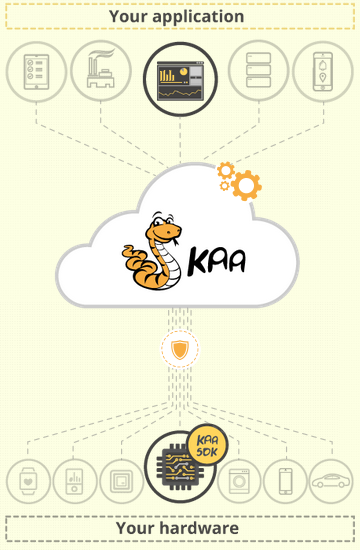
\includegraphics[scale=0.60]{../images/kaa/arqui.png}
		\caption{Arquitectura de KAA}
    \label{fig:kaalog}
	\end{center}
\end{figure}


\newpage

\subsection{Dispositivo receptor}

En éste aspecto no había muchas dudas en cuanto a las tecnologías a usar. Por una parte tenemos Raspbian, el sistema operativo oficial de Raspberry Pi basado en Debian. Usar algún otro sistema operativo ARM implicaría la incertidumbre sobre cualquier tipo de error en gran parte por el aspecto de los drivers.

\bigskip
Por otra parte tenemos el software desarrollado que se ejecuta en el dispositivo. Al igual que con el sistema operativo, el lenguaje de programación elegido desde un principio fué \textbf{Python} por su sencillez y número de bibliotecas. A medida que el desarrollo ha ido evolucionando Python ha demostrado ser el mejor candidato para el uso que se le pretendía dar, en gran parte gracias a la biblioteca \textbf{SoundDevice} que nos proporciona una manera realmente fácil de acceder y capturar datos de las interfaces de audio además de contar con numerosos ejemplos los cuales han sido de gran ayuda.

\bigskip
Por último, el dispositivo necesita hacer uso del SDK generado por KAA. Existen varias alternativas a la hora de generarlo y la más atractiva resultó ser \textbf{Java}. La interacción entre Python y Java se detallará más adelante.

\subsection{Almacenamiento de información}

Para almacenar datos de manera masiva existen varias alternativas como son Apache HBase, MongoDB, Apache Cassandra, Hive ó Redis. En éste aspecto la diferencia entre unas y otras es menores sin embargo hay una de ellas que destaca respecto a las otras por la facilidad de integración con KAA, es \textbf{Apache Cassandra} (\url{http://cassandra.apache.org/}).

\begin{figure}[!ht]
  \begin{center}
    
\includegraphics[scale=0.60]{../images/cassandra/logo.jpg}
    \label{fig:cassalog}
	\end{center}
\end{figure}

\begin{quote}\textit{ ''... is the right choice when you need scalability and high availability without compromising performance. Linear scalability and proven fault-tolerance on commodity hardware or cloud infrastructure make it the perfect platform for mission-critical data... is best-in-class, providing lower latency for your users...''
}
\newline
\url{http://cassandra.apache.org/}
\end{quote}

Tras una breve documentación acerca de Cassandra se vió que era un software con unas características y una potencia a tener muy en cuenta además de su facilidad integración con KAA como se ha mencionado anteriormente, también se pueden definir funciones personalizadas en el lenguaje deseado y tiene una línea de comandos amigable. El lenguaje de consultas es CQL y su sintaxis no difiere mucho del resto de SGBD.


\subsection{Representación de información}

En éste apartado las opciones a tener en cuenta era Apache-Zeppelin y Jupyter. Ambas herramientas tienen el papel de representar la información que va a almacenar Cassandra. La integración entre la base de datos y Zeppelin se hace de una manera sencilla así como las consultas y visualización de datos, es por eso por lo que finalmente se optó por la opción de \textbf{Apache Zeppelin} (\url{https://zeppelin.apache.org/}).

\begin{figure}[!ht]
  \begin{center}
    
\includegraphics[scale=0.60]{../images/zeppelin/logo.png}
    \label{fig:zepplog}
	\end{center}
\end{figure}

\begin{quote}\textit{ ''. A web-based notebook that enables interactive data analytics.
You can make beautiful data-driven, interactive and collaborative documents with SQL, Scala and more.''
}
\newline
\url{https://zeppelin.apache.org/}
\end{quote}

Apache Zeppelin nos va a permitir configurar una serie de Notebooks en forma de plataforma web en los que podremos realizar consultas a Cassandra para obtener los datos almacenados de los dispositivos receptores. Los datos se obtendrán mediante consultas CQL y podrán ser representados de varias formas, incluyendo distintos tipos de gráficos así como permitiendo la exportación de los mismos.

\subsection{Plataforma Web de RSMap}

Para la plataforma web aunque las opciones eran varias, la tecnología usada será Django que es un framework para aplicaciones web en Python.

\begin{figure}[!ht]
  \begin{center}
    
\includegraphics[scale=0.1]{../images/web/django-logo.png}
    \label{fig:drflog}
	\end{center}
\end{figure}

Las principales causas para la elección son la familiaridad con el mismo, que trabaja bajo el modelo vista-controlador, su documentación y el módulo Django-Rest-Framework que permite a los dispositivos comunicarse directamente con la web que será la encargada de representar en un mapa pequeños iconos que indiquen el paso de un vehículo.

El aspecto visual queda resuelto gracias a la librería Bootstrap.

\section{Instalación y configuración de Raspberry Pi}

\subsection{Instalación}

En primer lugar se indica como instalar Raspbian en nuestra Raspberry Pi Jessie (basado en Debian), ésta ha sido la opción seleccionada como SO debido a que es el sistema oficial que provee Raspberry Pi.

\bigskip

El primer paso es descargarse la imagen de los servidores oficiales, la imagen usada se puede encontrar en \url{https://downloads.raspberrypi.org/raspbian/images/raspbian-2016-05-31/}

\begin{lstlisting}[language=bash,caption={Copia de Raspbian en tarjeta s y usb},label={lst:pi1}]
# muestra los discos del sistema
$ lsblk
# copia la imagen en el dispositivo /dev/sdb (tarjeta sd)
$ sudo dd bs=1M if=2016-05-27-raspbian-jessie.img of=/dev/sdb
# copia la particion del sistema en /dev/sdc (usb)
$ sudo dd bs=1M if=/dev/sdb2 of=/dev/sdc
\end{lstlisting}

\bigskip

Ahora editamos el archivo \textbf{/dev/sdb/boot/cmdline.txt} y añadimos la siguiente línea para que el sistema sólo use la tarjeta SD para arrancar y el dispositivo usb como disco del sistema, ésto aumentará la velocidad de lectura considerablemente:


\begin{lstlisting}[language=bash,caption={Modificando el dispositivo de arranque de Raspbian},label={lst:pi2}]
smsc95xx.turbo_mode=N dwc_otg.lpm_enable=0 console=ttyAMA0,115200 kgdboc=ttyAMA0,115200 console=tty1 root=/dev/sda1 rootfstype=ext4 elevator=noop rootwait # /dev/sda1 point to our USB drive
\end{lstlisting}

\bigskip

\subsection{Configuración}

Vamos a instalar el software necesario para interactuar con la tarjeta de sonio además de comprobar si el sistema la soporta y en caso afirmativo, establecerla como dispositivo de audio por defecto lo cual nos permitirá trabajar con ella después de cada reinicio ó apagado del dispositivo.

\begin{lstlisting}[language=bash,caption={Instalación del paquete alsa-utils},label={lst:pi3}]
$ sudo apt-get install alsa-utils
\end{lstlisting}

\begin{lstlisting}[language=bash,caption={Comprobano que el dispositivo es reconocido},label={lst:pi3}]
$ lsusb
Bus 001 Device 005: ID 0d8c:000c C-Media Electronics, Inc. Audio Adapter
Bus 001 Device 004: ID 0781:5567 SanDisk Corp. Cruzer Blade
Bus 001 Device 003: ID 0424:ec00 Standard Microsystems Corp. SMSC9512/9514 Fast Ethernet Adapter
Bus 001 Device 002: ID 0424:9514 Standard Microsystems Corp.
Bus 001 Device 001: ID 1d6b:0002 Linux Foundation 2.0 root hub
\end{lstlisting}

\begin{lstlisting}[language=bash,caption={Identificando los dispositivos de sonido disponibles en el sistema},label={lst:pi4}]
$ aplay -l
**** List of PLAYBACK Hardware Devices ****
card 0: ALSA [bcm2835 ALSA], device 0: bcm2835 ALSA [bcm2835 ALSA]
  Subdevices: 8/8
  Subdevice #0: subdevice #0
  Subdevice #1: subdevice #1
  Subdevice #2: subdevice #2
  Subdevice #3: subdevice #3
  Subdevice #4: subdevice #4
  Subdevice #5: subdevice #5
  Subdevice #6: subdevice #6
  Subdevice #7: subdevice #7
card 0: ALSA [bcm2835 ALSA], device 1: bcm2835 ALSA [bcm2835 IEC958/HDMI]
  Subdevices: 1/1
  Subdevice #0: subdevice #0
card 1: Set [C-Media USB Headphone Set], device 0: USB Audio [USB Audio]
  Subdevices: 1/1
  Subdevice #0: subdevice #0
	\end{lstlisting}

\bigskip

En éste caso el dispositivo se llama \textit{C-Media USB Headphone SetC-Media USB Headphone Set} cuyo identificador es 1, para establecerla como dispositivo de audio por defecto editamos \textit{/home/user/.asoundrc} con el siguiente contenido:


\begin{lstlisting}[language=bash,caption={Comprobano que el dispositivo es reconocido},label={lst:pi5}]
    pcm.!default {
      type hw
      card 1
  }

  ctl.!default {
      type hw
      card 1
  }
\end{lstlisting}

\section{Instalación y configuración de KAA}

\subsection{Instalación}

Para la instalación de KAA nos bastará con Amazon EC2, ya que el sistema de imágenes de SO contiene la versión más actual de KAA, los pasos a seguir son los siguientes:

Necesitamos una cuenta en Amazon EC2, tras registrarnos nos dirigimos al panel principal, y en el apartado \textit{INSTANCES} seleccionamos, \textit{Launch Instance} para crear una nueva máquina.

\begin{figure}[!ht]
  \begin{center}
    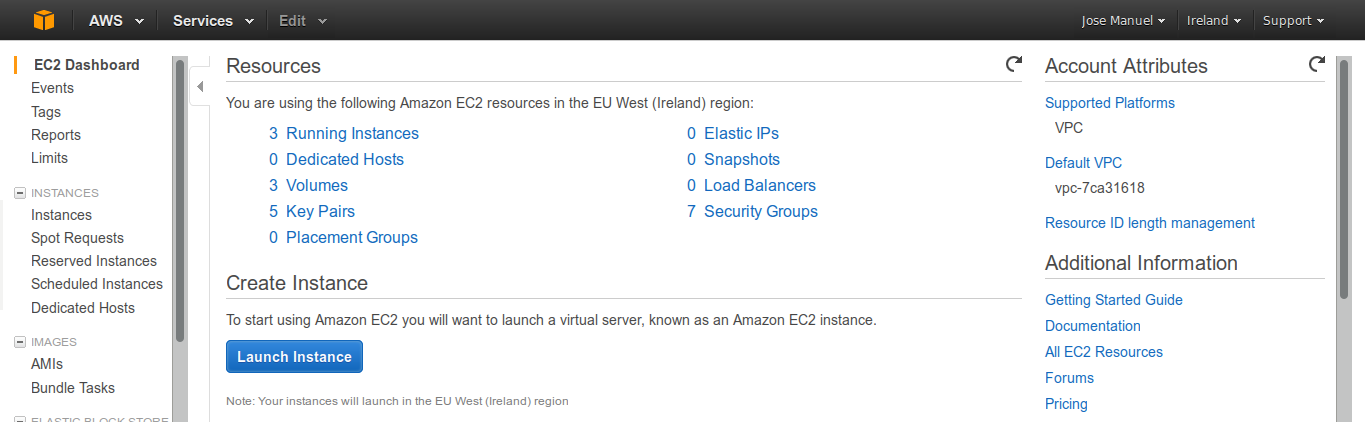
\includegraphics[scale=0.30]{../images/kaa/1.png}
		\caption{Dashboard de AmazonEC2}
    \label{fig:1}
	\end{center}
\end{figure}

El segundo paso es dirigirse a \textit{Community AMIs} y en el cuadro de búsqueda escribimos \textit{kaa-sandbox}. Lo recomendable es usar la última versión, en éste caso se ha tomado la \textbf{versión 0.9}.

\begin{figure}[!ht]
  \begin{center}
    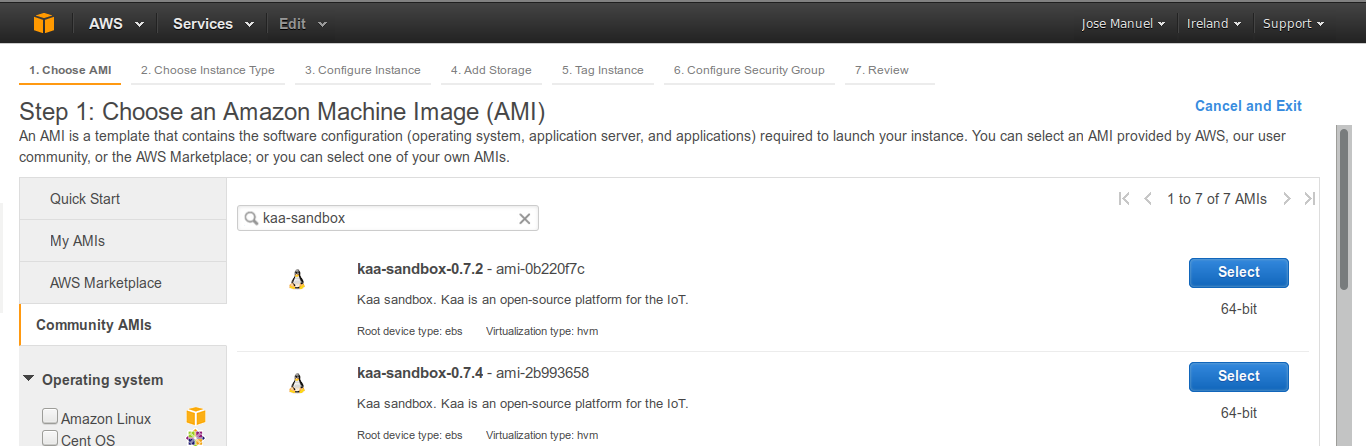
\includegraphics[scale=0.30]{../images/kaa/2.png}
		\caption{}
    \label{Instancias preconfiguradas de Kaa en EC2}
	\end{center}
\end{figure}

\newpage

Ahora debemos elegir el tipo de instancia, esto va directamente relacionado con la potencia de la misma. En un principio nos puede valer con las instancias de tipo \textit{free tier} y configurar la escalabilidad a medida de nuestras necesidades.

\begin{figure}[!ht]
  \begin{center}
    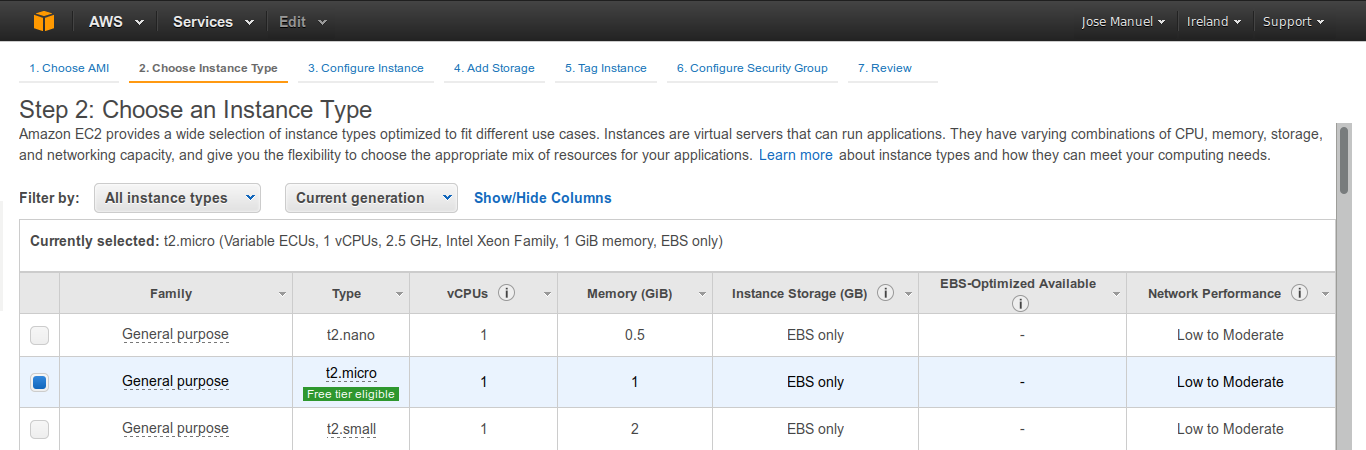
\includegraphics[scale=0.30]{../images/kaa/3.png}
		\caption{Selección del tipo de instancia}
    \label{fig:kaa}
	\end{center}
\end{figure}

En el siguiente paso podemos configurar algunas opciones relativas a la máquina, las que están por defecto son adecuadas por tanto no es necesario cambiar ninguna de ellas.

\begin{figure}[!ht]
  \begin{center}
    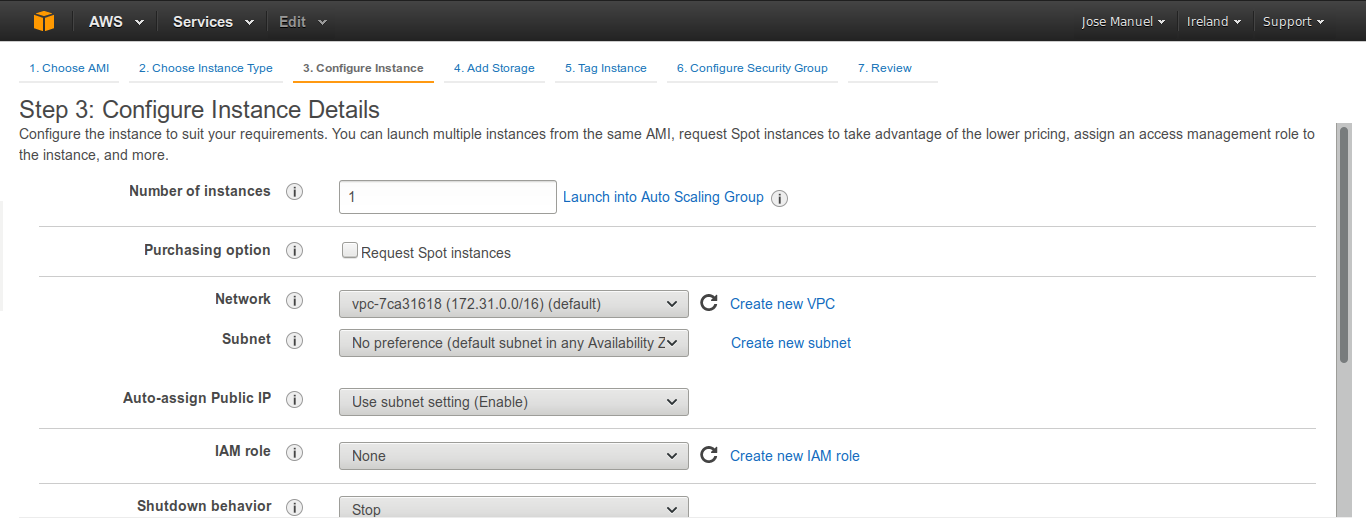
\includegraphics[scale=0.30]{../images/kaa/4.png}
		\caption{Configurar detalles de la instancia}
    \label{fig:kaa}
	\end{center}
\end{figure}

\newpage

El siguiente diálogo nos da la opción de configurar el almacenamiento, debido a que trabajamos en una instancia de tipo \textit{free tier} estamos restringidos a un tipo determinado de almacenamiento que al igual que el tipo de instancia, es suficiente por el momento.

\begin{figure}[!ht]
  \begin{center}
    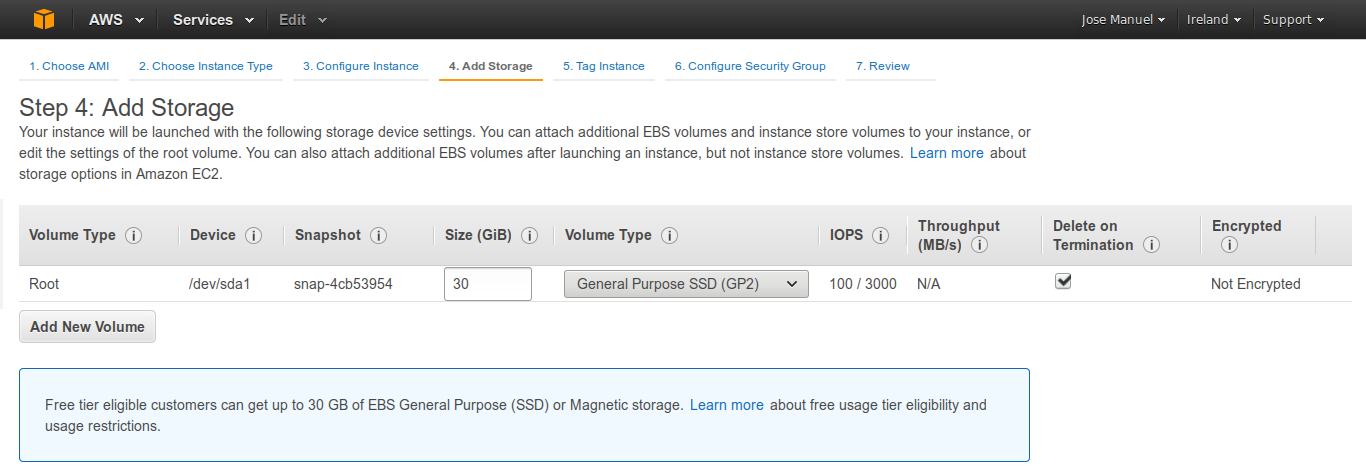
\includegraphics[scale=0.30]{../images/kaa/5.png}
		\caption{Selección de almacenamiento}
    \label{fig:kaa}
	\end{center}
\end{figure}

Los \textit{Security group} hacen referencia a la configuración de puertos, en la documentación de KAA se especifica cual debe ser, para el correcto funcionamiento y tiene una estructura como la de la \textit{ figura 6.7}.

\begin{figure}[!ht]
  \begin{center}
    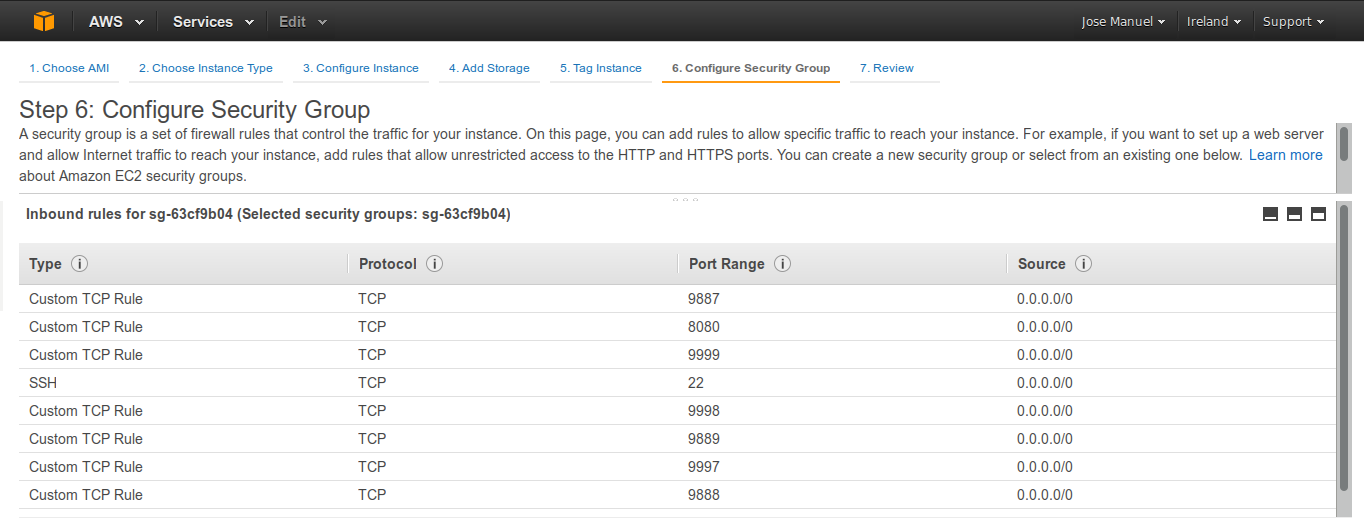
\includegraphics[scale=0.30]{../images/kaa/6.png}
		\caption{Configuración de puertos}
    \label{fig:kaa}
	\end{center}
\end{figure}

\newpage

Por último y no menos importante, debemos crear un par de llaves ó asignar uno existente. Ésto nos va a permitir conectarnos através de \textit{SSH} a la máquina en cualquier momento, si perdemos este par de claves perderemos el acceso a la máquina.

\begin{figure}[!ht]
  \begin{center}
    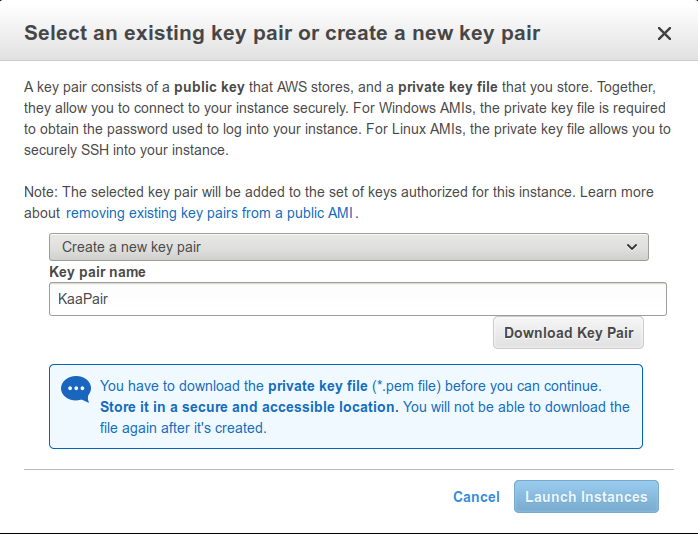
\includegraphics[scale=0.45]{../images/kaa/7.png}
		\caption{Creación de claves}
    \label{fig:kaa}
	\end{center}
\end{figure}

\subsection{Configuración}

Una vez tenemos el servicio instalado la configuración es trivial debido a que KAA provee un servicio web através del que definimos todo lo necesario.

Antes de empezar merece la pena destacar que existe 3 tipos de usuarios en KAA:

\begin{itemize}
	\item \textbf{Admin: } puede dar de alta Tenant admins.
	\item \textbf{Tenant admin: } puede dar de alta aplicaciones y Tenant developers.
	\item \textbf{Tenant developer:} puede configurar las aplicaciones y generar SDK's.
\end{itemize}

\bigskip

El primer paso es establecer la ip pública de KAA, accediendo desde el menú \textit{management}.

\begin{figure}[!ht]
  \begin{center}
    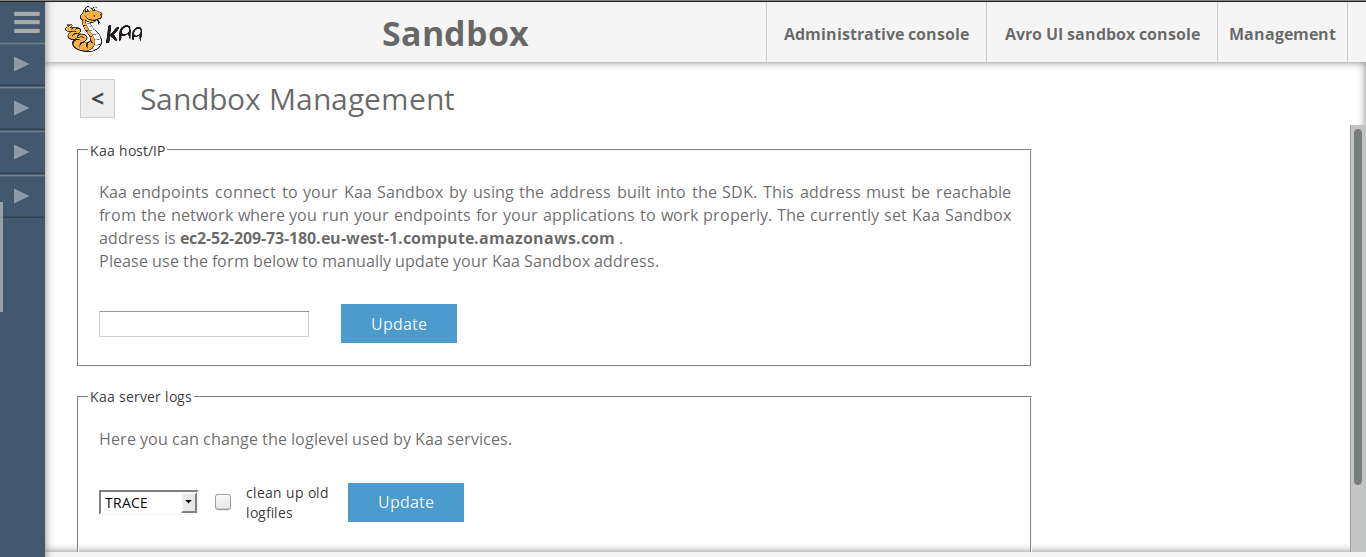
\includegraphics[scale=0.30]{../images/kaa/8.png}
		\caption{Sección Management}
    \label{fig:kaa}
	\end{center}
\end{figure}

\newpage

Ahora nos dirigimos a \textit{Administrative console} y nos logeamos como Tenant admin para dar de alta una nueva aplicación.

El tipo de credencial seleccionado será \textit{Trusful} de esta forma permitiremos a cualquier cliente conectarse a nuestra aplicación sin necesidad de autentificarse.

\begin{figure}[!ht]
  \begin{center}
    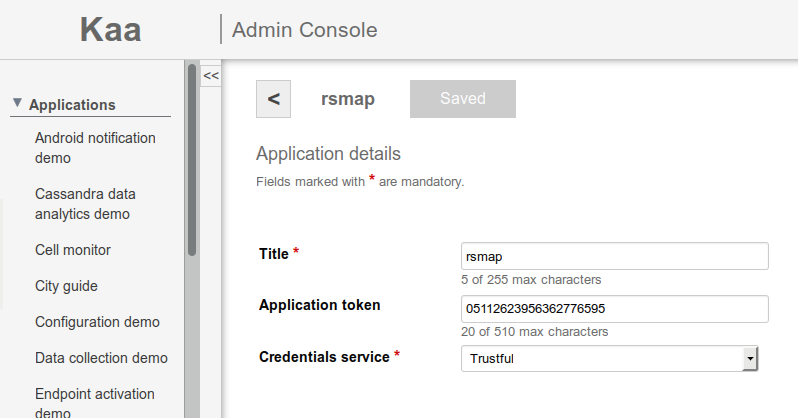
\includegraphics[scale=0.50]{../images/kaa/11.png}
		\caption{Creación de la nueva aplicación}
    \label{fig:kaa}
	\end{center}
\end{figure}

Nos logeamos con una cuenta Tenant Developer, vamos a proceder a crear la estructura de datos que define los campos y el tipo de los mismos que pertenecerán a nuestra aplicación.

Éste paso puede hacerse desde la interfaz web o subiendo un archivo \textit{json}. En nuestro caso vamos a valernos del \textit{json} por comodidad.

\begin{figure}[!ht]
  \begin{center}
    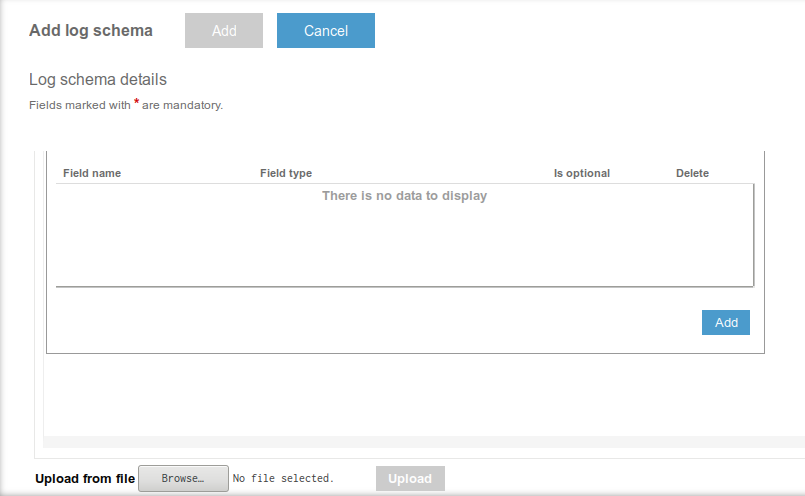
\includegraphics[scale=0.45]{../images/kaa/11-2.png}
		\caption{Definiendo esquemas de datos}
    \label{fig:kaa}
	\end{center}
\end{figure}

\newpage

El campo \textit{namespace} indica en que paquete se encontrará la clase correspondiente al esquema definido dentro del SDK generado.

\begin{lstlisting}[language=json,caption={Esquema de datos en JSON},label={lst:json_personal}]
{
	"type" : "record",
	"name" : "AudioReport",
	"namespace" : "org.kaaproject.kaa.schema.rsmap",
	"fields" : [ {
		"name" : "timestamp",
		"type" : "long"
	}, {
		"name" : "zoneId",
		"type" : {
			"type" : "string",
			"avro.java.string" : "String"
		}
	}, {
		"name" : "deviceId",
		"type" : {
			"type" : "string",
			"avro.java.string" : "String"
		}
	}, {
		"name" : "level",
		"type" : "double"
	} ]
}
\end{lstlisting}

Ahora ya tenemos el esquema definido en KAA como muestran la \textit{figura 6.12} y la \textit{figura 6.13}:

\begin{figure}[!ht]
  \begin{center}
    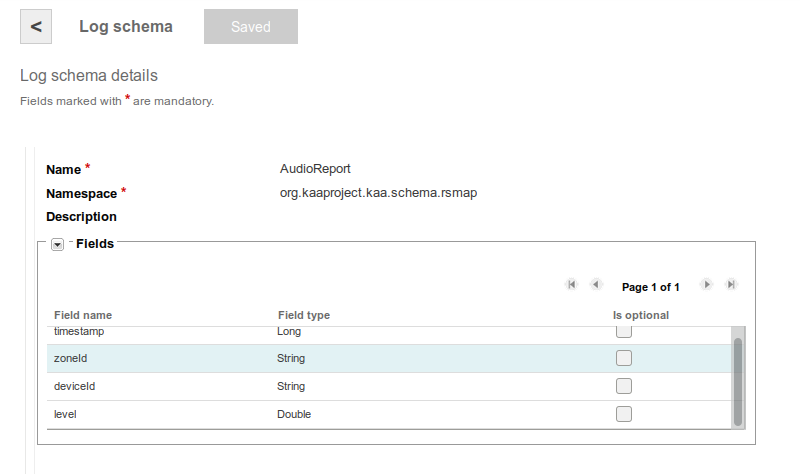
\includegraphics[scale=0.45]{../images/kaa/13.png}
		\caption{Esquema de datos definido 1}
    \label{fig:kaa}
	\end{center}
\end{figure}

\begin{figure}[!ht]
  \begin{center}
    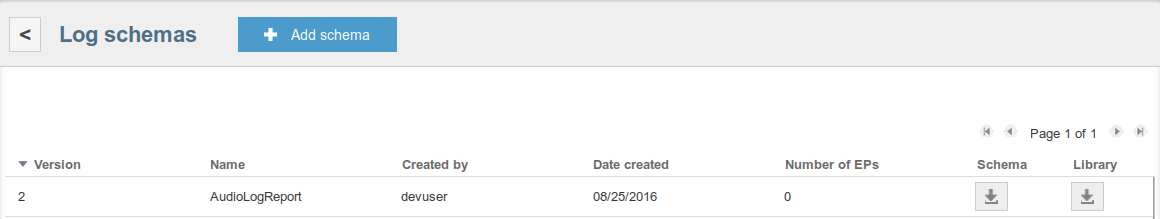
\includegraphics[scale=0.30]{../images/kaa/14.png}
		\caption{Esquema de datos definido 2}
    \label{fig:kaa}
	\end{center}
\end{figure}

\newpage

\newpage
\newpage
\newpage

\section{Instalación y configuración de Apache Cassandra.}

\subsection{Instalación}

El proceso para definir la máquina virtual que contiene Cassandra es el mismo que el de KAA a excepción de dos puntos, el primero es el tipo de instancia. Dentro de \textit{Community AMIs} debemos buscar \texit{Cassandra} y elegir la versión más reciente.

\begin{figure}[!ht]
  \begin{center}
    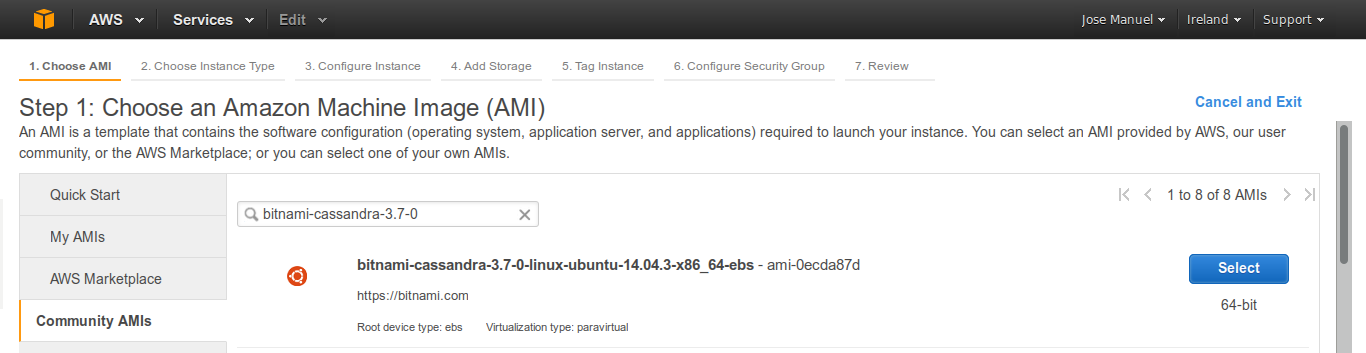
\includegraphics[scale=0.30]{../images/cassandra/1.png}
		\caption{Imagen de Cassandra en EC2}
    \label{fig:kaa}
	\end{center}
\end{figure}

El otro punto que difiere es el \textit{Security Group}, dado que los puertos que necesitamos son distintos la configuración debe quedar tal que así:

\begin{figure}[!ht]
  \begin{center}
    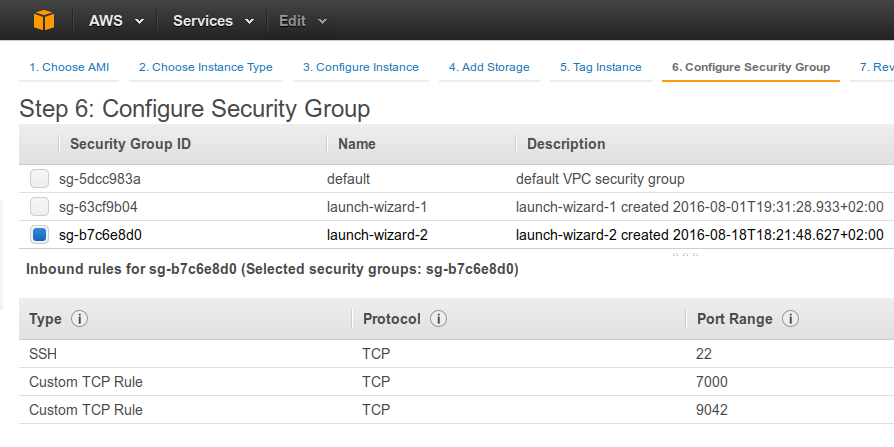
\includegraphics[scale=0.30]{../images/cassandra/2.png}
		\caption{Security Group para Cassandra}
    \label{fig:kaa}
	\end{center}
\end{figure}

\subsection{Configuración}

Para comprobar que funciona correctamente accedemos mediante \textit{SSH} y nos logeamos en la shell de Cassandra haciendo uso del comando \textbf{cqlsh} como indica la \textit{figura 6.16}.

\begin{figure}[!ht]
  \begin{center}
    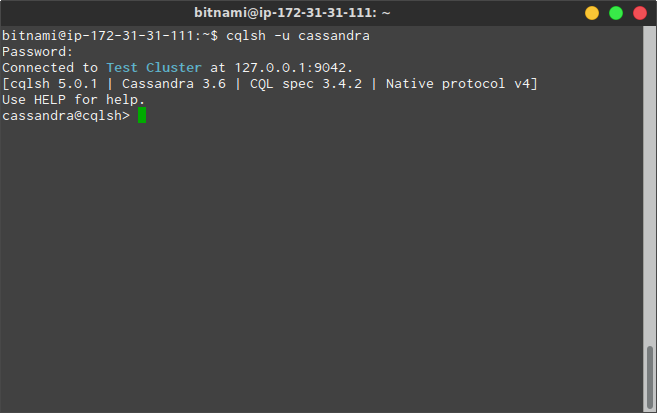
\includegraphics[scale=0.65]{../images/cassandra/3.png}
		\caption{Accediendo al servidor de Cassandra}
    \label{fig:kaa}
	\end{center}
\end{figure}

\newpage

Vamos a crear un \textit{Keyspace} que contendrá las tablas de nuestra aplicación, para ello usamos la siguiente sentencia:

\begin{lstlisting}[language=json,caption={Keyspace en Cassandra},label={lst:json_personal}]

CREATE KEYSPACE rsmapv0 WITH replication = {
	'class': 'SimpleStrategy',
	'replication_factor': 1
};

\end{lstlisting}

\textit{SingleStrategy} indica que sólo usaremos un \textit{Datacenter} y en \textit{replication factor} se indica el número de nodos de copia que queremos establecer.

\newpage

Ahora es momento de volver a KAA y definir el \textit{LogAppender} que se encargará de decirle a los clientes cómo y donde tienen que enviar los datos mediante el SDK. En nuestro caso será la base de datos que acabamos de configurar. Ésto lo haremos en la sección de Log appenders mediante un fichero \textit{json} con la siguiente estructura:


\begin{lstlisting}[language=json,caption={Esquema de log appender en JSON},label={lst:json_personal}]

{
   "cassandraServers":[
      {
         "host":"ec2-52-210-20-84.eu-west-1.compute.amazonaws.com",
         "port":9042
      }
   ],
   "cassandraCredential":{
      "org.kaaproject.kaa.server.appenders.cassandra.config.gen.CassandraCredential":{
         "user":"####",
         "password":"####"
      }
   },
   "keySpace":"rsmapv0",
   "tableNamePattern":"rows",
   "columnMapping":[
      {
         "type":"EVENT_FIELD",
         "value":{
            "string":"zoneId"
         },
         "columnName":"zone_Id",
         "columnType":"TEXT",
         "partitionKey":true,
         "clusteringKey":false
      },
      {
         "type":"EVENT_FIELD",
         "value":{
            "string":"timestamp"
         },
         "columnName":"timestamp",
         "columnType":"BIGINT",
         "partitionKey":false,
         "clusteringKey":true
      },
      {
         "type":"EVENT_FIELD",
         "value":{
            "string":"deviceId"
         },
         "columnName":"device_Id",
         "columnType":"TEXT",
         "partitionKey":false,
         "clusteringKey":true
      },
      {
         "type":"EVENT_FIELD",
         "value":{
            "string":"level"
         },
         "columnName":"level",
         "columnType":"DOUBLE",
         "partitionKey":false,
         "clusteringKey":false
      }
   ],
   "clusteringMapping":[
      {
         "columnName":"timestamp",
         "order":"DESC"
      }
   ],
   "cassandraBatchType":{
      "org.kaaproject.kaa.server.appenders.cassandra.config.gen.CassandraBatchType":"UNLOGGED"
   },
   "cassandraSocketOption":null,
   "executorThreadPoolSize":1,
   "callbackThreadPoolSize":2,
   "dataTTL":0,
   "cassandraWriteConsistencyLevel":{
      "org.kaaproject.kaa.server.appenders.cassandra.config.gen.CassandraWriteConsistencyLevel":"ONE"
   },
   "cassandraCompression":{
      "org.kaaproject.kaa.server.appenders.cassandra.config.gen.CassandraCompression":"NONE"
   },
   "cassandraExecuteRequestType":{
      "org.kaaproject.kaa.server.appenders.cassandra.config.gen.CassandraExecuteRequestType":"SYNC"
   },
   "minLogSchemaVersion":1,
   "maxLogSchemaVersion":2147483647,
   "pluginTypeName":"Cassandra",
   "pluginClassName":"org.kaaproject.kaa.server.appenders.cassandra.appender.CassandraLogAppender",
   "headerStructure":[

   ]
}

\end{lstlisting}

\newpage

Los detalles a destacar son que el usuario y la contraseña de Cassandra han sido ocultados por seguridad. Otro punto importante es que aquí se define a donde queremos enviar los datos mediante la IP pública del servidor Cassandra.
Los campos del final indican la equivalencia entre los campos de esquema creado anteriormente y las tablas en Cassandra.

Un factor importante es el diseño de las tablas, pues las consultas en Cassandra son dependientes de la estructura de la base de datos. El tipo de campos que determinan la estructura de la tabla son los siguientes:

\begin{itemize}
\item \textbf{partitionKey, } que es la responsable de la distribución de los datos entre los nodos de Cassandra.
\item \textbf{clusteringKey, } que se usa para ordenar los elementos dentro de una partición.
\end{itemize}

En el caso de RSMap se usa el campo \textit{zoneId} como \textit{partition key} y \textit{timestamp y deviceId} como \textit{clustering key} lo que nos garantiza que podremos hacer consultas del tipo:


\begin{lstlisting}[language=cql,caption={Mécanica de consultas en CQL según la estructura de tablas},label={lst:json_personal}]

SELECT * FROM abc WHERE partitionKey = 'X';
SELECT * FROM table WHERE partitionKey = 'X' AND clusteringKey  = 'Y';

\end{lstlisting}

\bigskip

Tras guardar el \textit{log appender} podemos comprobar como se ha creao la tabla \textit{rows} dentro del keyspace \textit{rsmapv0}. Para realizar ésta comprobación accedemos a la shell de Cassandra como muestra la \textit{figura 6.17	}.

\begin{figure}[!ht]
  \begin{center}
    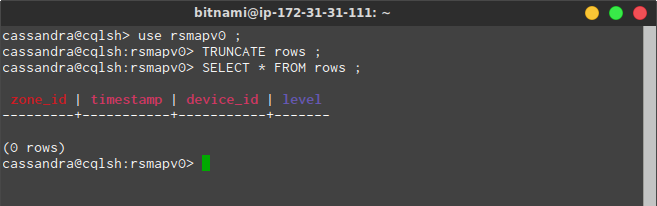
\includegraphics[scale=0.65]{../images/cassandra/4.png}
		\caption{Comprobación de las tablas creadas}
    \label{fig:kaa}
	\end{center}
\end{figure}

Para finalizar vamos a crear dos funciones en java dentro del Keyspace, las cuales nos ayudarán a visualizar y consultar los datos posteriormente. Es importante destacar que estas funciones pueden ser definidas en el lenguaje que queramos, en nuestro caso vamos a usar Java.

\bigskip

La primera convierte un \textit{timestamp} en una hora legible, las otras dos nos ayudarán a seleccionar los datos de un minuto atrás hasta la fecha actual y de una hora atrás hasta la fecha actual.

\begin{figure}[!ht]
  \begin{center}
    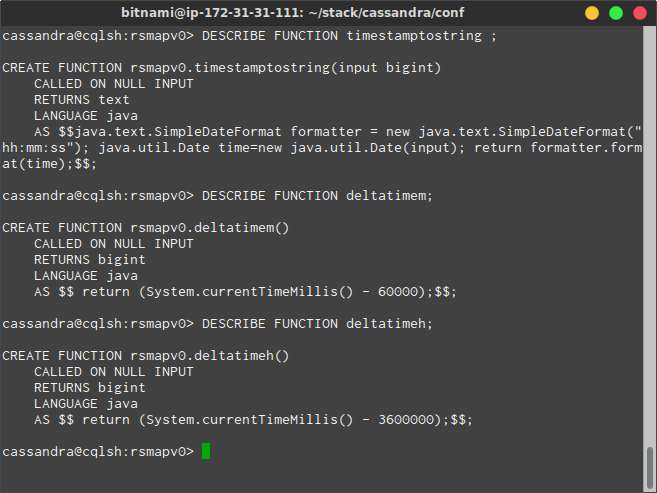
\includegraphics[scale=0.65]{../images/cassandra/5.png}
		\caption{Funciones dentro de Cassandra}
    \label{fig:kaa}
	\end{center}
\end{figure}

\newpage

Si queremos hacer uso de éstas funciones debemos editar el fichero \textbf{/home/bitnami/stack/cassandra/conf} y cambiar la línea:

enable user defined functions: false

por:

enable user defined functions: true

\bigskip

Ya sólo nos queda reiniciar el servicio:

\begin{lstlisting}[language=bash,caption={Reiniciando Cassandra},label={lst:rcas}]
	$ sudo ./stack/ctlscript.sh stop cassandra
	$ sudo ./stack/ctlscript.sh start cassandra
\end{lstlisting}

\newpage

\section{Desarrollo del módulo de sonido.}
TO CLEAN AND INSERT HERE
\newpage


\section{Desarrollo de la plataforma web.}
TO CLEAN AND INSERT HERE
\newpage


\section{Instalación y configuración de Apache Zeppelin.}

\subsection{Instalación}
Es hora de instalar Apache-Zeppelin. Como en los servicios anteriores, lo primero que debemos hacer es configurar e iniciar una nueva instancia en Amazon EC2. Los pasos a seguir son los mismos con la salvedad de la selección de la imagen y la configuración de \textit{Security groups}.

\bigskip

La SO usado esta vez será Ubuntu 14.04.4 LTS, para seleccionarlo lo podemos buscar dentro de las imágenes disponibles al configurar la nueva instancia.

Como tráfico entrante abriremos el puerto 8080 que es donde se va a ejecutar Apache-Zeppelin.

Una vez que tengamos la máquina disponible accedemos por SSH y procedemos a instalar Apache-Zeppelin con las siguientes órdenes:

\begin{lstlisting}[language=bash,caption={Instalación de Apache-Zeppelin},label={lst:pi1}]
$ cd /opt
$ sudo wget http://apache.rediris.es/zeppelin/zeppelin-0.6.1/zeppelin-0.6.1.tgz
$ sudo tar -zxvf zeppelin-0.6.1.tgz
$ sudo /opt/zeppelin-0.6.1-bin-all/zeppelin-daemon.sh
\end{lstlisting}

Debemos asegurarnos de descargar el binario que trae los intérpretes instalados, entre ellos el de Cassandra para poder hacer llamadas a la base de datos en los Notebooks.

Si ahora abrimos el navegador a nuestra dirección pública deberíamos encontrarnos con lo siguiente:

\begin{figure}[!ht]
  \begin{center}
    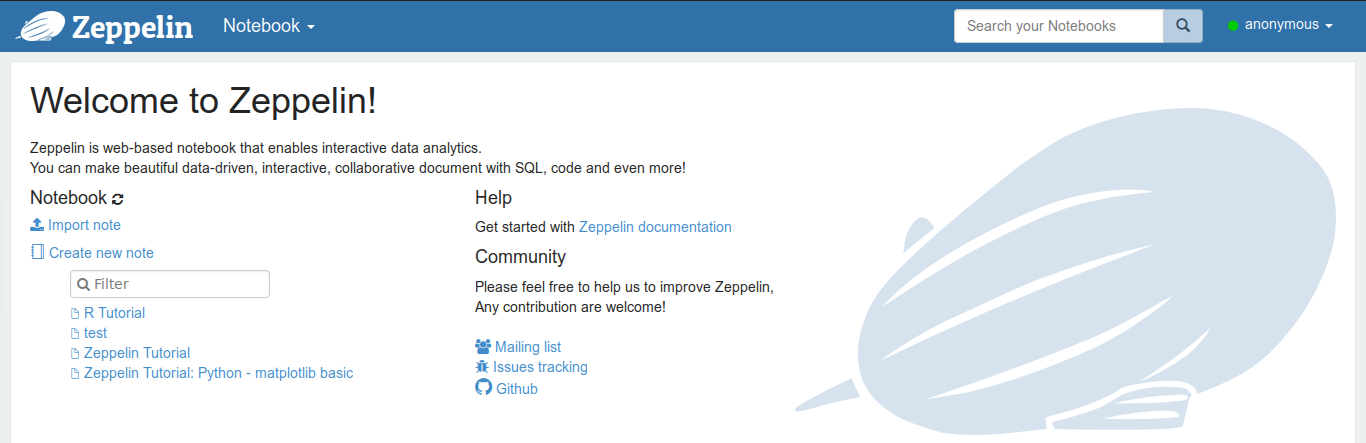
\includegraphics[scale=0.30]{../images/zeppelin/1.png}
		\caption{Apache Zeppelin en funcionamiento}
    \label{fig:kaa}
	\end{center}
\end{figure}

\subsection{Configuración}

Vamos a configurar es el intérprete de Cassandra, para ello nos dirigimos a la parte derecha de la interfaz y entramos en la opción \textit{interpreters}. Tras localizar el intérprete de Cassandra pulsamos el botón \textit{editar} y configuramos los siguientes campos:

\begin{itemize}
\item \textbf{cassandra.credentials.password, } aquí indicamos la contraseña de Cassandra.
\item \textbf{cassandra.credentials.username, } aquí el usuario.
\item \textbf{cassandra.hosts, } aquí la dirección pública del servidor de Cassandra.
\item \textbf{cassandra.keyspace , } y aquí el Keyspace que definimos anteriormente en Cassandra.
\end{itemize}

para finalizar guardamos los cambios efectuados.

Ahora estamos preparados para crear un nuevo Notebook para RSMap mediante el menú desplegable \textit{Notebooks} y la opción \textit{create new notebook} al cual deberemos establecer un nombre. Una vez hecho ésto entraremos en el Notebook que tiene una estructura como muestra la \textit{figura 6.20}.

\begin{figure}[!ht]
  \begin{center}
    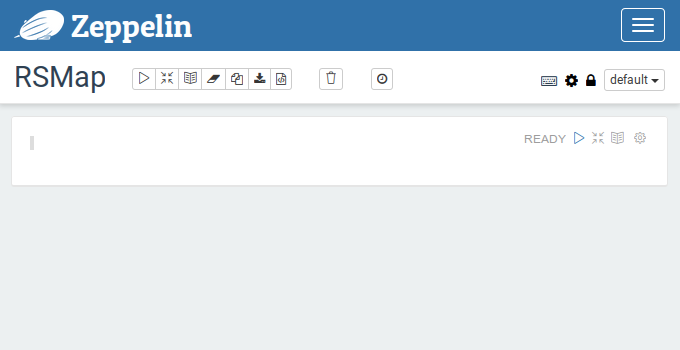
\includegraphics[scale=0.50]{../images/zeppelin/2.png}
		\caption{Estructura de un Notebook en Zeppelin}
    \label{fig:kaa}
	\end{center}
\end{figure}

Sólo queda una tarea por realizar, que es configurar cuales de los intérpretes estarán disponibles para usar bajo este Notebook.
Existen muchos como el de \textit{Scala, Python, Java o Markdown} entre otros.

Para configurarlos nos dirigimos a la rueda dentada situada en la parte derecha y desactivamos todos los intérpretes a excepción de el de Cassandra. La configuración debe quedar tal que así:

\begin{figure}[!ht]
  \begin{center}
    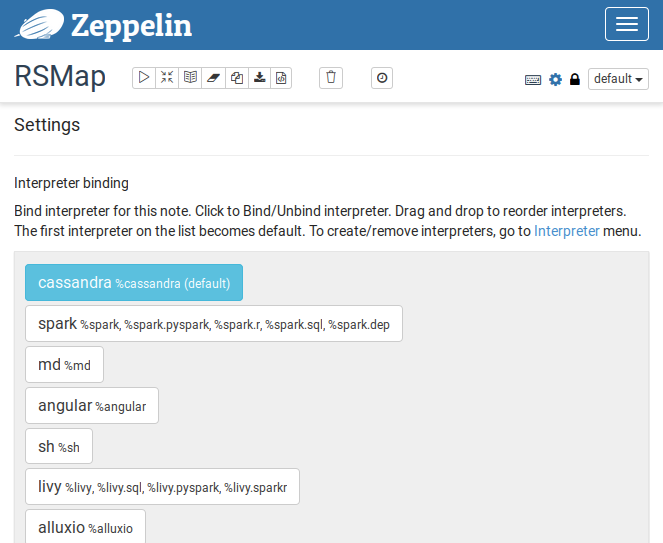
\includegraphics[scale=0.50]{../images/zeppelin/3.png}
		\caption{Cassandra como intérprete para Zeppelin}
    \label{fig:kaa}
	\end{center}
\end{figure}

\newpage

Ya tenemos todos los elementos preparados para realizar consultas en \textit{CQL} a nuestro servidor Cassandra y poder visualizar los datos. La interfaz de Zeppelin está compuesta de varias celdas en las cuales podemos introducir el código deseado.

En nuestro caso estas sentencias pertenecen al intérprete de Cassandra luego la primera línea de cada celda debe contener la palabra clave \textbf{\%cassandra}. Una vez tengamos escrita la consulta podemos pulsar el botón de \textit{Play} y esperar unos segundos para obtener los resultados.

\bigskip

Vale la pena destacar que Zeppelin posee un sistema de programación de tareas al que podemos acceder pulsando el pequeño icono del reloj llamado \textit{Run scheduler} con una estructura similar a crontab, ésto nos permite programar un tiempo predeterminado para que se ejecuten las celdas del Notebook de manera automática y poder tener los resultados actualizados en todo momento.

\subsection{Ejemplo de consulta CQL}

Detallamos un ejemplo de consulta a modo de ilustración de como funciona CQL, veamos que forma tiene y posteriormente se comentarán las diferentes partes de la misma.

\begin{lstlisting}[language=cql,caption={Ejemplo de consulta CQL},label={lst:json_personal}]
%cassandra
SELECT rsmapv0.timestampToString(timestamp) AS time, level from rsmapv0.rows WHERE zone_id={{zone_id='Granada'}} and timestamp > rsmapv0.deltatimeH() ORDER BY timestamp ASC;
\end{lstlisting}

Como se vió en la parte de configuración de Cassandra habíamos creado ciertas funciones para usarlas a la hora de consultar los datos, es el momento de verlas en funcionamiento. \textit{rsmapv0.timestampToString} es la función que nos formatea un \textit{timestamp} a una fecha, rsmapv0 indica en que Keyspace se encuentra dicha función.

En la cláusula WHERE tenemos \textbf{ zone id = \{\{zone id='Granada'\}\}} lo que nos permitirá modificar el valor de ese campo mediante la interfaz de Zeppelin si necesidad de reescribir la consulta.

En último lugar \textbf{rsmapv0.deltatimeH()} hace referencia a una de las otras funciones definidas en Cassandra, en este caso se indica en la consulta que el campo \textit{timestamp} debe ser mayor que \textbf{rsmapv0.deltaTimeH}. Ésta función nos devuelve la hora actual restándole un minuto, por tanto obtendremos todos los valores de un minuto antes de la fecha actual.

\bigskip

Tras poner el sistema en funcionamiento durante un minuto en el que pasan algunos vehículos podemos ver como Zeppelin representa los datos mediante la consulta mencionada:

\begin{figure}[!ht]
  \begin{center}
    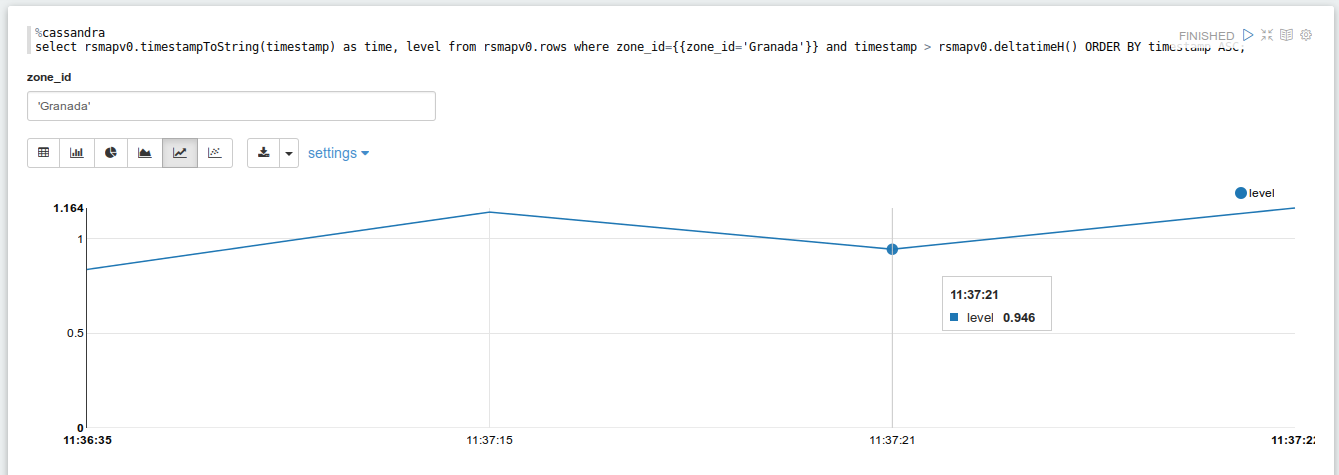
\includegraphics[scale=0.30]{../images/zeppelin/4.png}
		\caption{Muestra de resultados en Zeppelin}
    \label{fig:kaa}
	\end{center}
\end{figure}

\newpage
